\documentclass[11pt,a4paper]{article}
\usepackage[margin=2.5cm]{geometry}
\usepackage{booktabs}
\usepackage{enumitem}
\usepackage{hyperref}
\usepackage{tikz}
\usetikzlibrary{arrows.meta}

\title{Rubik's Cube fNIRS -- Experimental Protocol (Pilot)}
\author{Adam Aske}
\date{Version 0.1 -- \today}

\begin{document}
\maketitle

\section{Aim}
Track re-learning of the 3$\times$3 Rubik's Cube in a single subject (the author) over
repeated sessions, while recording haemodynamic activity with fNIRS over the
prefrontal cortex (planning, working memory) and the occipital cortex (visual
processing). The behavioural outcomes are planning time and solve time per
trial; the imaging outcome is the block-wise HbO/HbR response in the
\textsc{Plan} and \textsc{Solve} blocks relative to rest.

This document describes the pilot protocol. It is expected to change after the
pilot and discussion with colleagues; keep the version number and date updated.

\section{Setup}
\begin{itemize}[nosep]
  \item fNIRS system with optodes over prefrontal and occipital cortex, recorded in
        Aurora (or equivalent) with an LSL marker stream enabled.
  \item Subject seated at a table, cube placed on the table in front of them.
  \item Trigger PC running \texttt{scripts/run\_session.py}, which opens an LSL
        outlet named \texttt{Trigger} (type \texttt{Markers}, one \texttt{int32} channel).
        Select this stream in the acquisition software before starting.
  \item The subject operates the script themselves (single-subject pilot): the
        ENTER key advances self-paced blocks. Keep the keyboard within reach of
        the non-dominant hand and press ENTER with the cube already down/up as
        instructed, so keypresses do not add to the measured times.
\end{itemize}

\section{Block design}
One \emph{trial} is one solve. Each trial consists of the blocks in
Table~\ref{tab:blocks}; trials are separated by a break during which the subject
scrambles the cube using the scramble printed by the script. A session consists
of at least 5 trials.

\begin{table}[h]
\centering
\caption{Blocks of one trial.}
\label{tab:blocks}
\begin{tabular}{l l l p{7cm}}
\toprule
Block & Duration & Marker & Instruction \\
\midrule
\textsc{Rest (pre)}  & 20 s & 10 & Sit still, eyes open, look at the (scrambled) cube on the table. Do not touch it. \\
\textsc{Plan}        & self-paced & 20 & Pick up the cube and inspect it. Plan the first step(s). No turns allowed. Press ENTER at the moment of the first turn. \\
\textsc{Solve}       & self-paced & 30 & Solve the cube. When solved, put it down and press ENTER. Type \texttt{d} then ENTER if the solve failed (DNF). \\
\textsc{Rest (post)} & 45 s & 40 & Sit still, eyes open, look at the cube on the table. \\
\textsc{Break}       & $\geq$ 120 s & 50 & Relax, then scramble the cube with the printed scramble. Put it down and press ENTER to start the next trial. \\
\bottomrule
\end{tabular}
\end{table}

\begin{center}
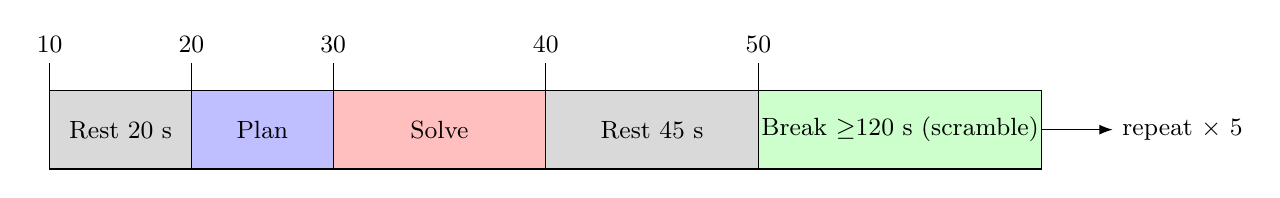
\begin{tikzpicture}[x=0.9cm, every node/.style={font=\small}]
  \foreach \x/\w/\name/\col in {0/2/Rest 20 s/gray!30, 2/2/Plan/blue!25, 4/3/Solve/red!25, 7/3/Rest 45 s/gray!30, 10/4/Break $\geq$120 s (scramble)/green!20} {
    \draw[fill=\col] (\x,0) rectangle (\x+\w,1) node[midway]{\name};
  }
  \draw[-{Latex}] (14,0.5) -- (15,0.5) node[right]{repeat $\times$ 5};
  \foreach \x/\m in {0/10, 2/20, 4/30, 7/40, 10/50} {
    \draw (\x,1) -- (\x,1.35); \node[above] at (\x,1.35) {\m};
  }
\end{tikzpicture}
\end{center}

\subsection*{Timing notes}
\begin{itemize}[nosep]
  \item The pre-trial rest is short (20 s) because the post-trial rest of the
        previous trial plus the break already provide a long baseline; it mainly
        serves as an immediate pre-stimulus baseline.
  \item The post-trial rest is 45 s so the haemodynamic response of the solve can
        return towards baseline before the subject moves to scramble.
  \item Planning time and solve time are derived from the marker timestamps
        ($t_{30}-t_{20}$ and $t_{40}-t_{30}$) and also saved by the script.
\end{itemize}

\section{Trigger table}
Markers are integers pushed on the LSL stream. The table is defined in
\texttt{scripts/triggers.py} and reproduced here (regenerate with
\texttt{python scripts/make\_tables.py}). Tens digit = phase, ones digit = sub-event.

\begin{center}
\begin{tabular}{r l p{8.5cm}}
\toprule
Code & Name & Meaning \\
\midrule
  1 & \texttt{SESSION\_START} & Session begins; recording should already be running \\
  2 & \texttt{SESSION\_END} & Session ends; stop the recording after this \\
  10 & \texttt{REST\_PRE} & Pre-trial rest onset (eyes open, cube on table, 20 s) \\
  20 & \texttt{PLAN} & Planning/inspection onset: subject picks up the cube and inspects, no turning \\
  30 & \texttt{SOLVE} & Solve onset: first turn allowed. Also marks end of PLAN \\
  40 & \texttt{REST\_POST} & Post-trial rest onset: cube put down. Also marks end of SOLVE (solve time = t40 - t30) \\
  50 & \texttt{BREAK} & Inter-trial break onset (2 min). Subject scrambles the cube during this \\
  60 & \texttt{DNF} & Trial flagged as not properly solved / aborted by the subject \\
  99 & \texttt{ABORT} & Session aborted by the experimenter \\
\bottomrule
\end{tabular}

\end{center}

Only block \emph{onsets} are marked; the end of a block is the onset of the next.
Marker 60 (DNF) is pushed immediately after marker 40 for the same trial.

\section{Session procedure}
\begin{enumerate}[nosep]
  \item Mount the cap, check signal quality, start the recording in Aurora.
  \item Start the script: \texttt{python scripts/run\_session.py --subject 1 --trials 5}.
        The session number auto-increments from \texttt{data/sessions.csv}.
  \item Verify the \texttt{Trigger} stream is visible and selected in Aurora.
  \item Scramble the cube with the first scramble the script prints, put it down,
        press ENTER. Marker 1 is sent and the first trial starts.
  \item Follow the on-screen instructions for each block.
  \item After the last trial, marker 2 is sent. Stop the recording, then save the
        raw fNIRS data to \texttt{data/raw/} using the log name printed by the
        script (e.g. \texttt{sub-01\_ses-01\_YYYYMMDD\_HHMMSS}).
  \item Run \texttt{python scripts/make\_tables.py} and rebuild \texttt{report/report.tex}.
\end{enumerate}

\section{Data produced per session}
\begin{itemize}[nosep]
  \item \texttt{logs/<name>.json} -- all parameters, every marker with wall-clock and LSL
        timestamps, per-trial scramble, plan time, solve time, break length, DNF flag.
  \item \texttt{logs/<name>.log} -- plain-text log of the same.
  \item \texttt{data/solves.csv} -- one row appended per solve (across sessions).
  \item \texttt{data/sessions.csv} -- one row appended per session (the ``completed protocols'' table).
  \item \texttt{data/raw/} -- fNIRS recordings (not in git).
\end{itemize}

\section{Open questions for after the pilot}
\begin{itemize}[nosep]
  \item Should \textsc{Plan} be capped (e.g. 15 s WCA-style inspection) to make it a fixed-length block?
  \item Is the break long enough for the signal to settle after scrambling (a motor task)?
  \item Add a control task (e.g. random turning without solving) to separate motor from cognitive activity?
  \item Eyes-closed vs eyes-open rest; fixation cross instead of looking at the cube?
  \item Number of trials per session vs fatigue and cap comfort.
\end{itemize}

\end{document}
